\section{Memory Disaggregation}

\begin{figure*}[h!]
    \centering
    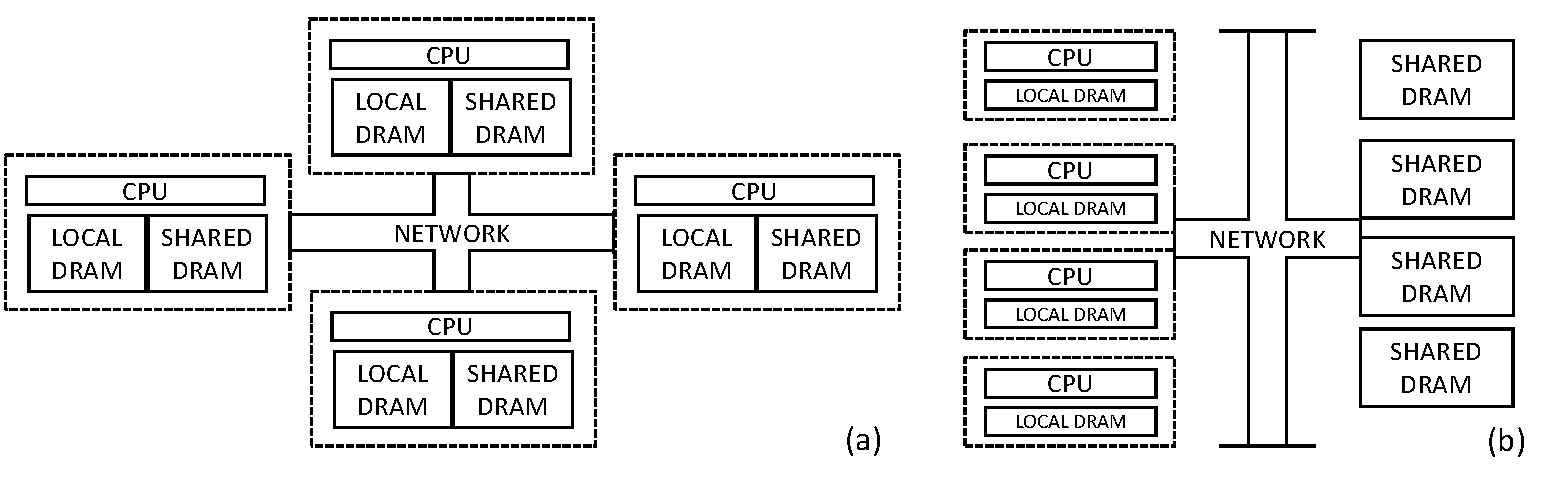
\includegraphics[width=.9\linewidth]{fig/architecture.pdf}
    \caption{Shows (a) software-disaggregated 
    architecture where disaggregated memory is pooled from 
    traditional servers as opposed to the (b) hardware-disaggregated
    design where most memory is decoupled in hardware.}
    \label{fig:architecture}
\end{figure*}

Memory disaggregation aims to decouple the available compute 
and memory resources in the cluster and allow for independent 
allocations of these resources regardless of where a job 
is placed. This means, the OS/runtime 
that's running the job should provide a platform to 
expose/give access to potentially all the memory 
available in the cluster. Ideally, it should hide the 
complexity of setting up and accessing remote memory 
(e.g., RDMA connection setup) and 
expose an easy-to-use interface for working with remote memory.
At the same time, it should trade-off the properties 
of the interface with decent performance guarantees 
and other requirements from the system like resource 
sharing and isolation across applications. At a high 
level, the platform is a distributed system consisting 
of a client-side (compute-side) components (a runtime 
that exposes the memory interface and acts as an agent 
on each compute node), the server-side (memory) components 
(to manage memory on each memory server) and an 
interconnect over which these components interact to 
provide an abstraction for shared cluster memory.
It may optionally include other cluster resources like
centralized managed for global memory/metadata management
and failure handling.

\vspace{3pt}
\noindent \uline{Target Architecture.}
Proposed solutions for memory disaggregation target two 
different kind of cluster/memory architectures based on
existing technologies or technologies that are expected
to be available in the near future (shown in 
Figure ~\ref{fig:architecture}).

% \begin{itemize}
%     \item 
\vspace{3pt}
\noindent \textbf{1. Software-disaggregated.}
Some systems~\cite{gms,cashmere,infiniswap,remregions,
leap,zswap} target the traditional homogeneous 
datacenters with monolithic servers as the basic 
deployment unit, connected to each other by low-latency 
network interconnects like Infiniband or RoCE. Each 
unit hosts both compute and memory resources and the 
software provides an interface to remote memory 
on other nodes. Local memory is prioritized for 
local jobs and unutilized memory on all the nodes 
can be pooled and presented to the cluster as 
remote/disaggregated memory, which could be static 
or vary in capacity over time. 

    % \item 
\vspace{3pt}
\noindent \textbf{2. Hardware-disaggregated.}
Other systems~\cite{kona,aifm,fastswap,semeru,legoos} 
target a hardware disaggregated architecture where (most 
of the) memory nodes are detached from the compute nodes 
and made available through the network. The memory node 
can be a traditional monolithic server with limited 
compute and stuffed with DRAM~\cite{fastswap} or 
each DRAM unit itself directly-attached to a memory 
controller and network interface~\cite{legoos}. 
Even in a purely disaggregated setup, however, 
it is generally assumed that each compute node has 
a small amount of local memory and vice 
versa.~\cite{legoos,kona}
% \end{itemize}

In both architectures, compute servers use the local memory 
to run the OS and other runtime essentials for exposing remote 
memory, and only use remote memory for the applications. 
There are many reasons for this choice. 
First, without local DRAM, all the memory 
accesses would be remote and the memory controller should 
possess the knowledge and capability to fetch remote memory 
directly without any help from software; such complex ``control 
path" knowledge would need either a ``smart" memory controller 
(e.g., RMC in soNUMA~\cite{sonuma}) or some other smart 
hardware (e.g., ccFPGA in Kona~\cite{kona}) next to it. 
Even these solutions do not put OS on remote memory and 
and maintain local DRAM to exploit cache locality as remote 
accesses are still worse than local.

{\renewcommand{\arraystretch}{1.2}% for the vertical row padding
\begin{table*}[!t]
    \centering
    \begin{tabular}{l|ccccc} 
        % \hline         
        \textbf{\shortstack[l]{Interface Type \\ (Implementation)}}
            & \textbf{System}
            & \textbf{Transparent}
            & \textbf{General}
            & \textbf{\shortstack[c]{What can be\\Remote}}
            & \textbf{\shortstack[c]{Sharing \\ support}}
        \\ \hline
        \multirow{4}{*}{\shortstack[l]{Virtual Memory \\ (Traditional Paging)}}
            & Infiniswap~\cite{infiniswap} (2017)
            & Yes
            & Yes
            & All
            & No
        \\ \cline{2-6}
            & zSwap~\cite{zswap} (2019)
            & Yes
            & Yes
            & All
            & No
        \\ \cline{2-6}
            & Leap~\cite{leap} (2019)
            & Yes
            & Yes
            & All
            & No
        \\ \cline{2-6}
            & Fastswap~\cite{fastswap} (2020)
            & Yes
            & Yes
            & All
            & No
        \\ \hline
        \multirow{2}{*}{\shortstack[l]{Virtual Memory \\ (New Hardware)}}
            & LegoOS~\cite{legoos} (2018)
            & Yes
            & Yes
            & All
            & No
        \\ \cline{2-6}
            & Kona~\cite{kona} (2021)
            & Yes
            & Yes
            & Heap
            & No
        \\ \hline
        \multirow{2}{*}{\shortstack[l]{Language-based \\ (User space)}}
            & AIFM~\cite{aifm} (2020)
            & Yes
            & No
            & Portion
            & No
        \\ \cline{2-6}
            & Semeru~\cite{semeru} (2020)
            & Yes
            & No
            & (Java) Heap
            & No
        \\ \hline
        \multirow{2}{*}{\shortstack[l]{Custom API \\ (Kernel-based)}}
            & Remote Regions~\cite{remregions} (2020)
            & No
            & Yes
            & Portion
            & Basic
        \\ \cline{2-6}
            & LITE MRs~\cite{literdma} (2017)
            & No
            & Yes
            & Portion
            & Basic
        \\ \hline
        % FaRM~\cite{farm}
        %     & PGAS
        %     & User space
        %     & No
        %     & No
        %     & Portion
        %     & Yes
        % \\ \hline
        % GAM~\cite{gam}
        %     & PGAS
        %     & User space
        %     & No
        %     & No
        %     & Portion
        %     & Yes
        % \\ \hline
    \end{tabular}
    \vskip .5em
    \caption{Various interfaces for remote memory adopted in 
    some recent systems}
    \label{tab:interfaces}
  \end{table*}